\date{} \usepackage{usenix} \title{\Large \bf Reducing Data Center Latency}

for single author \author{ 
{\rm Zainab Ghadiyali}\\ Department of Computer
Science, University of Wisconsin-Madison 
\and {\rm Michael Griepentrog}\\
Department of Computer Science, University of Wisconsin-Madison 
\and{\rm Aditya Akella}\\
Department of Computer Science, University of Wisconsin-Madison
} 
% end author


\maketitle

% Use the following at camera-ready time to suppress page numbers.  Comment it
% out when you first submit the paper for review.
\thispagestyle{empty}


\subsection*{Abstract}

\section{Introduction} In the last few decades, the key focus of the network
comunnity has been on improving the overall goodput of networks. The initial
focus on circuit switching moved to packet switching due to bandwidth and
hardware inefficiences in working with reservations for network resources for
bursty communication traffic. The Transmission Control Protocol(TCP) was
invented to address the issue of bandwidth/congestion collapse in the network
and ensure bandwidth fairness.~\cite{DCTCP,Queueing,TCP_Pacing} However network
latency has been given less importance. Most applications are throughput
oriented (e.g. email) are not sensitive of delivary times and the latency for
latency sensitive applications is seen as an acceptable tradeoff in order to
maintain high bandwidth utilization.   
However, there is now an increasing interest in reducing latency in
datacenters. A substantial amount of computing is now shifting to data centers
and reducing latency is now easier given the confines of a building rather than
tackling the issue for the internet at large. Furthermore, ultra low latency
 sensitive applications such as High Frequency Trading, HPC and Google Instant 
Search service may especially benefit from this. 
Network Interface Cards (NIC), end-host stacks and switches are all points 
where a packet may experience latency while traversing from client to server. 
In order to address delays arising from queueing delay at switches, 
DCTCP ~\cite{DCTCP} uses ECN marking to slow down flows before the queue is 
saturated. HULL ~\cite{HULL} further suggests trading off a little bandwidth to 
provide smaller amount of latency.  
In this paper, we look into understanding how switch, various offloading
parameters and hardware influences latency.

OUR OBSERVATION IS THAT

THROUGH OUR EVALUATION WE FIND THAT

\section{Methodology}
A strong evaluation and understanding of reducing latency will be incomplete
without simulateneously studying the tradeoffs between latency and other
important factors such as bandwidth and CPU utilization. Thus, we study latency
along with its influence on CPU utilization and bandwidth. 

In order to understand latency influencing paramters, it is also essential to
understand the corresponding tradeoffs in throughput and CPU utilization. We
collect these metrics by running ping, iperf and pidtest. These metrics were
obtained for TCP and UDP flows, where each flow was subjected to various
TCP segmentation offload (TSO), Generic segmentation offload (GSO) and 
Generic segmentation offload (GRO) settings. Firstly, the effect of keeping
TSO/GSO and GRO settings on was evaluated. This was followed by studying the
effects of all setting off. Effect of TSO/GSO was evaluated by keeping these
parameters on while GRO was switched off. Similarly, effect of GRO was evaluated
by keeping the GRO paramater on, while TSO/GSO were switched off. 
 
\section{Evaluation}
\subsection{Bandwidth}
\begin{figure}[t] 
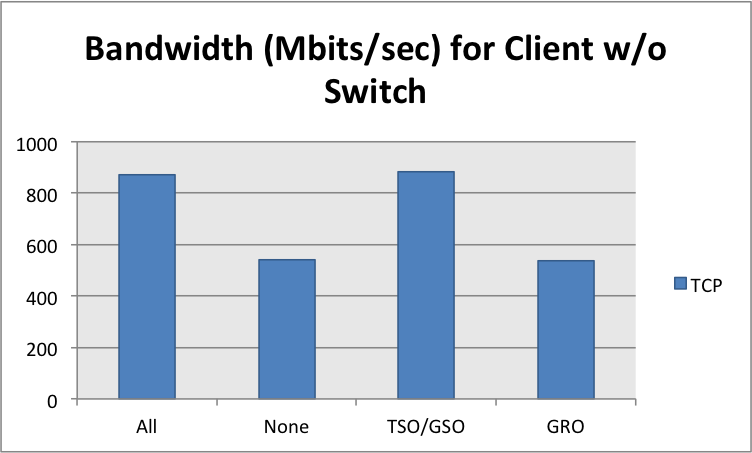
\includegraphics[scale=0.75]{avg_bandwidth_client_noswitch.png}
\caption{Bandwidth is halved when GRO or TSO/GSO/GRO is switched off} 
\label{fig:avg_bandwidth_client_noswitch}
\end{figure}

\begin{figure}[t] 
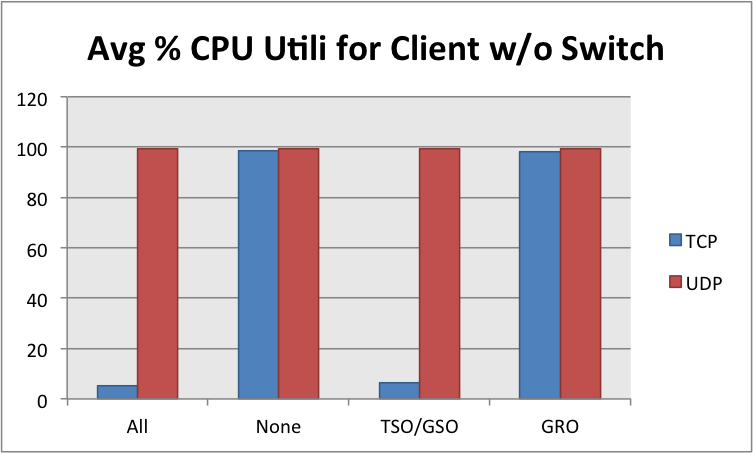
\includegraphics[scale=0.75]{avg_cpu_client_noswitch.png}
\caption{CPU utilization is maxed when GRO or TSO/GSO/GRO is switched off} 
\label{fig:avg_cpu_client_noswitch}
\end{figure}


\begin{figure}[t] 
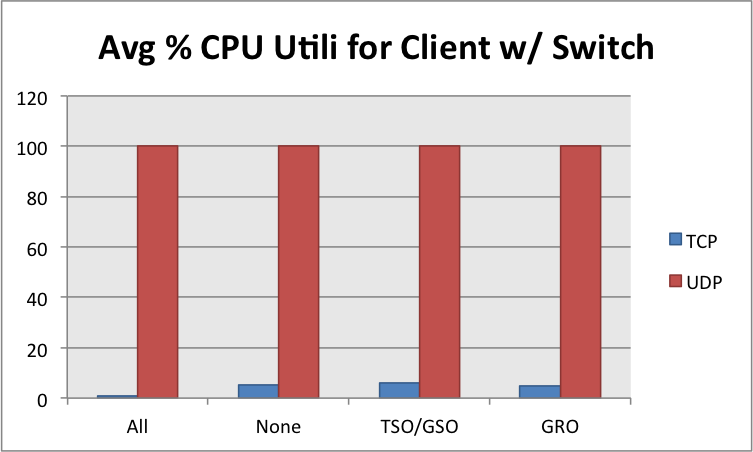
\includegraphics[scale=0.75]{avg_cpu_client_switch.png}
\caption{CPU utilization is not influenced by offloading settings 
in presence of switch} 
\label{fig:avg_cpu_client_switch}
\end{figure}


\begin{figure}[t] 
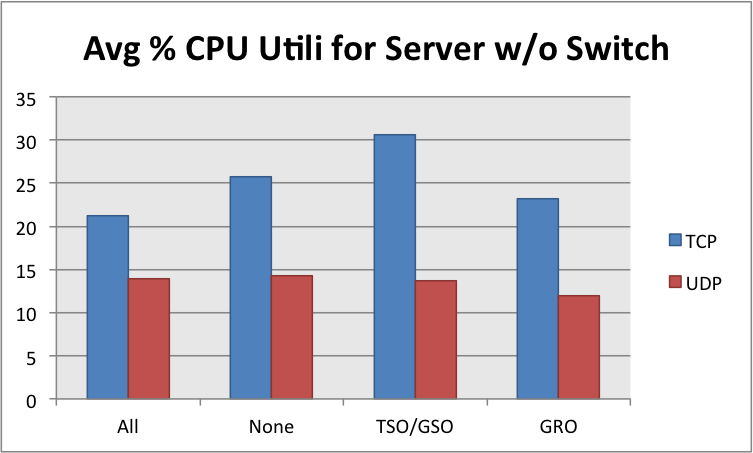
\includegraphics[scale=0.75]{avg_cpu_server_noswitch.png}
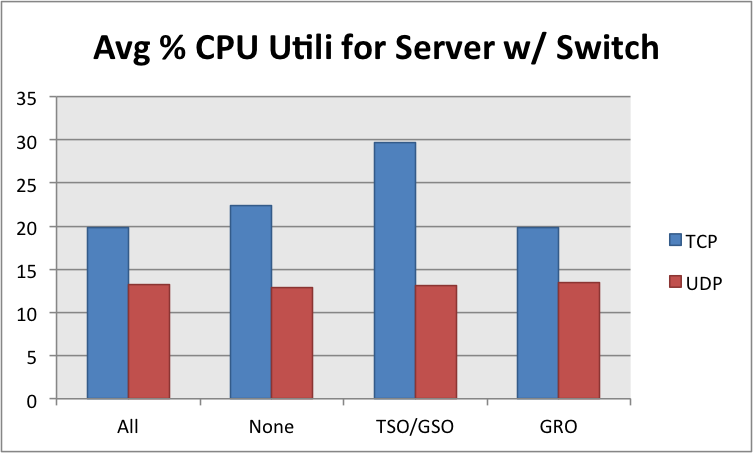
\includegraphics[scale=0.75]{avg_cpu_server_switch.png}
\caption{CPU utilization remains fairly evenly distributed at the server end
in the presence or absence of a switch} 
\label{fig:avg_cpu_server_noswitch}
\end{figure}

\begin{figure}[t] 
\includegraphics[scale=0.75]{avg_cpu_tcp_client.png}
\caption{CPU utilization may be influenced by absence of GRO or TSP/GSO/GRO on
the client side} 
\label{fig:avg_cpu_tcp_client}
\end{figure}

\begin{figure}[t] 
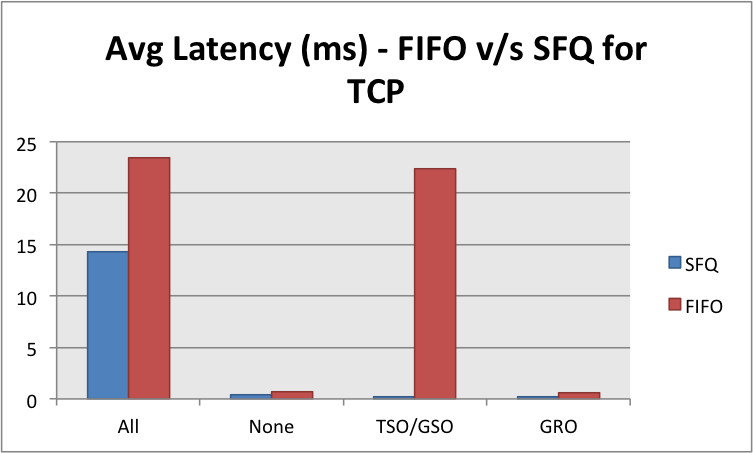
\includegraphics[scale=0.75]{avg_latency_fifo_sfq.png}
\caption{Latency remains unaffected in absence of GRO or TSO/GSO/GRO settings
off for FIFO as well as SFQ. A significant decrease in latency is observed for
SFQ in absence of all offloading parameters} 
\label{fig:avg_latency_fifo_sfq}
\end{figure}


\begin{figure}[t] 
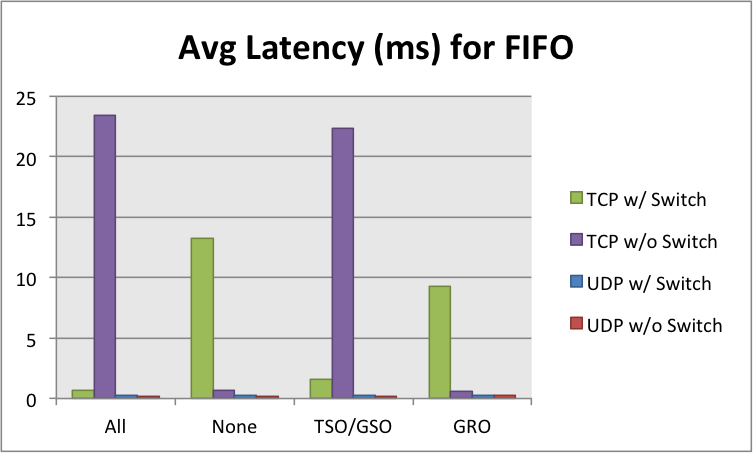
\includegraphics[scale=0.75]{avg_latency_FIFO.png}
\caption{Latency is higher for TCP thand UDP flows. Furthermore, latency is
higher for TCP flows in absense of switch} 
\label{fig:avg_latency_FIFO}
\end{figure}


\begin{figure}[t] 
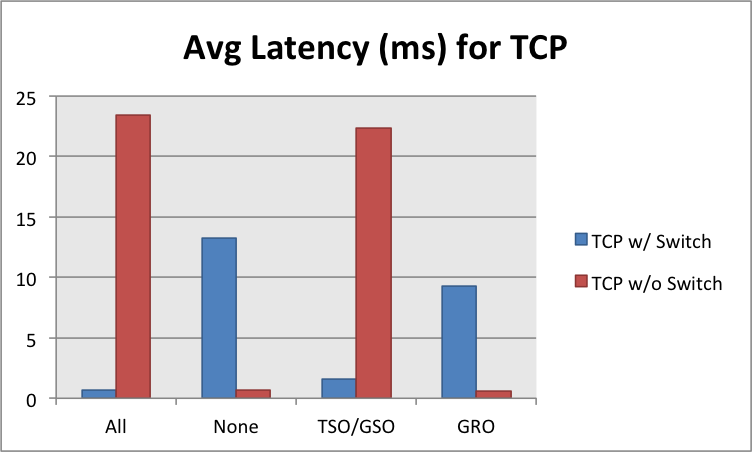
\includegraphics[scale=0.75]{avg_latency_tcp.png}
\caption{Latency is highest for TCP flows in the absense of a switch and
presense of all or only TSO/GSO} 
\label{fig:avg_latency_tcp}
\end{figure}


\begin{figure}[t] 
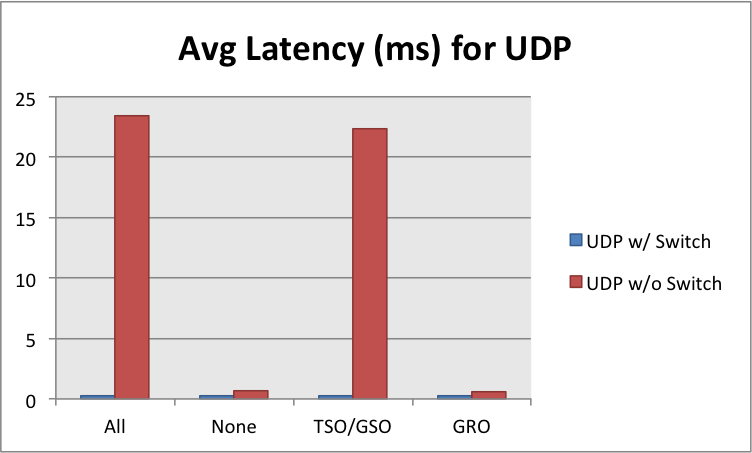
\includegraphics[scale=0.75]{avg_latency_udp.png}
\caption{Latency for UDP flows is highest in absence of a switch and presence of
all or only TSO/GSO presnece
} 
\label{fig:avg_latency_udp}
\end{figure}

\section{Conclusion}

\section{Acknowledgments}

We would like to thank Aaron Gember without whose help, running experiments on
the Open Flow test best at the University of Wisconsin-Madison would not be
possible.  


{\footnotesize \bibliographystyle{acm} \bibliography{

\bibitem{DCTCP} DCTCP Linux kernel patch. http://www.stanford.edu/alizade/Site/
DCTCP.html.
\bibitem{Queueing} A. Demers, S. Keshav, and S. Shenker. Analysis and simulation of a fair
queueing algorithm. In Proc. of SIGCOMM, pages 1–12, 1989.
\bibitem{TCP_Pacing} D.Lacamera. TCP Pacing Linux Implementation. http://danielinux.net/
index.php/TCP Pacing.
\bibitem{HULL}M. Alizadeh, A. Kabbani, T. Edsall, B. Prabhakar, A. Vahdat, and M. Yasuda. Less
Is More: Trading a Little Bandwidth for Ultra-Low Latency in the Data Center. In
Proceedings of USENIX
NSDI conference, 2012
}}


\theendnotes

\end{document}
